\chapter{Pokémon}
\label{chap:pokemon}
For purposes of battle, a Pokémon $P$ is defined as having:
\begin{itemize}
\item A species and form (and thus a typing and base stats)
\item An Individual Vector (IV) (\autoref{sec:ivs}) and level (\autoref{sec:plevel})
\item A set of two or three attacks, one of which is a fast attack
\item Shadow status, or the absence thereof
\item Some number of hit points {\symbolfont󰥽} MHP.
\end{itemize}
Visual presentation and size do not affect battle, nor does Purified status.
Hit Points are carried across PvE battles (including encounters with
  Team GO Rocket and Gym battles), but Trainer Battles always start with full HP\@.
A Pokémon with zero hit points has ``fainted''.
Fainted Pokémon cannot be used in battles of any kind, nor can they be left in
 Power Stops (see \autoref{sec:maxbattles}).

\section{Pokémon Level}
\label{sec:plevel}
Each Pokémon has its own level, taking one of the 99 integer and half-integer
 values between 0--50, inclusive.
A Trainer can ``power up'' their Pokémon in single level increments,
 not exceeding the Trainer's own level plus 10.
Each increase has a cost in Stardust and the Candy of that genus; beyond level 40, there
  is a further cost in Candy XL (\autoref{table:powerups}).
\begin{table}
  \footnotesize
  \begin{center}
    \begin{tabular}[ht]{rrrr|rrrr}
      Level &
        k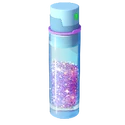
\includegraphics[width=1em,height=1em]{images/stardust.png} &
        
\includegraphics[width=1em,height=1em]{images/rarecandy.png} &
        
\includegraphics[width=1em,height=1em]{images/rarecandyxl.png} &
      Level &
        k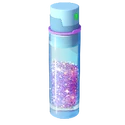
\includegraphics[width=1em,height=1em]{images/stardust.png} &
        
\includegraphics[width=1em,height=1em]{images/rarecandy.png} &
        
\includegraphics[width=1em,height=1em]{images/rarecandyxl.png} \\
      \Midrule\\\\
        1 & 0.2 & 1 & & 25.5 & 2.2 & 2 & \\
      1.5 & 0.2 & 1 & & 26 & 2.2 & 2 & \\
        2 & 0.2 & 1 & & 26.5 & 2.2 & 2 & \\
      2.5 & 0.2 & 1 & & 27 & 2.2 & 2 & \\
        3 & 0.2 & 1 & & 27.5 & 2.2 & 2 & \\
      3.5 & 0.2 & 1 & & 28 & 2.2 & 2 & \\
        4 & 0.2 & 1 & & 28.5 & 2.2 & 2 & \\
      4.5 & 0.2 & 1 & & 29 & 2.2 & 2 & \\
        5 & 0.2 & 1 & & 29.5 & 2.2 & 2 & \\
      5.5 & 0.2 & 1 & & 30 & 2.2 & 2 & \\
        6 & 0.2 & 1 & & 30.5 & 2.2 & 2 & \\
      6.5 & 0.2 & 1 & & 31 & 2.2 & 2 & \\
        7 & 0.2 & 1 & & 31.5 & 2.2 & 2 & \\
      7.5 & 0.2 & 1 & & 32 & 2.2 & 2 & \\
        8 & 0.2 & 1 & & 32.5 & 2.2 & 2 & \\
      8.5 & 0.2 & 1 & & 33 & 2.2 & 2 & \\
        9 & 0.2 & 1 & & 33.5 & 2.2 & 2 & \\
      9.5 & 0.2 & 1 & & 34 & 8 & 10 & \\
       10 & 0.2 & 1 & & 34.5 & 8 & 10 & \\
     10.5 & 0.2 & 1 & & 35 & 8 & 10 & \\
       11 & 0.2 & 1 & & 35.5 & 8 & 10 & \\
     11.5 & 0.2 & 1 & & 36 & 8 & 10 & \\
       12 & 0.2 & 1 & & 36.5 & 8 & 10 & \\
     12.5 & 0.2 & 1 & & 37 & 8 & 10 & \\
       13 & 0.2 & 1 & & 37.5 & 8 & 10 & \\
     13.5 & 0.2 & 1 & & 38 & 8 & 10 & \\
       14 & 0.2 & 1 & & 38.5 & 8 & 10 & \\
     14.5 & 0.2 & 1 & & 39 & 8 & 10 & \\
       15 & 0.2 & 1 & & 39.5 & 8 & 10 & \\
     15.5 & 0.2 & 1 & & 40 & 8 & 10 & \\
       16 & 0.2 & 1 & & 40.5 & 8 & 10 & \\
     16.5 & 0.2 & 1 & & 41 & 8 & 10 & \\
       17 & 0.2 & 1 & & 41.5 & 8 & 10 & \\
     17.5 & 2.2 & 2 & & 42 & 8 & 10 & \\
       18 & 2.2 & 2 & & 42.5 & 8 & 10 & \\
     18.5 & 2.2 & 2 & & 43 & 8 & 10 & \\
       19 & 2.2 & 2 & & 43.5 & 8 & 10 & \\
     19.5 & 2.2 & 2 & & 44 & 8 & 10 & \\
       20 & 2.2 & 2 & & 44.5 & 8 & 10 & \\
     20.5 & 2.2 & 2 & & 45 & 8 & 10 & \\
       21 & 2.2 & 2 & & 45.5 & 8 & 10 & \\
     21.5 & 2.2 & 2 & & 46 & 8 & 10 & \\
       22 & 2.2 & 2 & & 46.5 & 8 & 10 & \\
     22.5 & 2.2 & 2 & & 47 & 8 & 10 & \\
       23 & 2.2 & 2 & & 47.5 & 8 & 10 & \\
     23.5 & 2.2 & 2 & & 48 & 8 & 10 & \\
       24 & 2.2 & 2 & & 48.5 & 8 & 10 & \\
     24.5 & 2.2 & 2 & & 49 & 8 & 10 & \\
       25 & 2.2 & 2 & & 49.5 & 8 & 10 & \\
    \end{tabular}
  \end{center}
  \caption{Power-up costs per Pokémon levels}
  \label{table:powerups}
\end{table}
An increase in level improves the Pokémon's attack and defense, and
  will sometimes increase MHP.
See \autoref{chap:stats} for a quantitative treatment.

Powering up a fainted Pokémon will revive it, but with minimal HP\@:

\[ HP = \min{1, MHP_{New} - MHP_{Old} } \]

\section{Individual Vectors}
\label{sec:ivs}
Each Pokémon has three integers associated with it, each ranging from 0--15.
They are unchanging across the Pokémon's existence.

Once a Trainer has joined a team (\autoref{sec:levels}), the ``Appraise'' function can be used to
  get a visual representation of these three numbers (this representation,
  while annoying, is sufficient to determine the actual numbers).
Additionally, the Pokémon will be given a rating of 0--4, represented as
  one, two, or three stars (0 shows one star; 4 shows three, albeit in a different color).
A Pokémon rated 4 has an IV of 15/15/15, and is colloquially known as a ``hundo'' or ``100\%er''.
Such Pokémon have their own Pokédex (\autoref{sec:dexen}).
A Pokémon rated 0 has an IV of 0/0/0, and is colloquially known as a ``nundo'' or ``0\%er''.
They have no unique Pokédex, because they are worthless pieces of shit,
  and don't let anyone tell you otherwise\footnote{Consult \autoref{chap:optimal}
  to see that 0/0/0 is never an optimal IV.}.
While 15/15/15 is generally the optimal IV, this is not always true in CP-bounded
  competition; see \autoref{chap:bounded} for more information,
  and \autoref{chap:optimal} for tables of optimal IVs under different CP bounds.

\section{Generation of IV and level}
\label{sec:ivgeneration}
IVs and levels are generated when the Pokémon is ``created'', not when it is captured.
It is thus possible to glean information from the CP displayed for a Pokémon;
  one can sometimes even uniquely determine the IV\@.
The equation for CP is provided in \autoref{chap:unbounded}; reverse it and
  use \autoref{table:cpm} plus the base stats of the species to determine
  the set of IV+level pairs yielding that CP\@.
Various applications and websites can perform this analysis automatically.
Depending on the situation, there might be a floor for IVs.
Beyond that, they are uniformly randomly generated.
The chance of any given IV for a catch in the wild (without weather boosting)
  is exactly the same---1 out of 4096.
The probability of a random Pokémon being a hundo is actually
  greater than that of being a nundo, due to the existence of IV floors
  (e.g. the chance of a 15/15/15 for a lucky trade is 1 in 256, whereas
  a 0/0/0 is impossible).
\begin{table}
  \begin{center}
    \begin{tabular}{lcc}
      Context & IV floors & Level \\
      \Midrule \\
      \multirow{2}{*}{Wild catch} & 0 & 1--max(TL, 30) \\
      & 4 w/ weather boost & 1--max(TL, 30) + 5 \\
      Hatch & 10 & max(TL, 20) \\
      \multirow{2}{*}{Raid} & 10 & 20 \\
      & 6 (shadow) & 25 w/ weather boost \\
      Max Battle & 10 & 20 \\
      Research & 10 & 15 \\
      Team GO Rocket & 0 & 8 \\
      Grunts and Leaders & 4 w/ weather boost & 13 w/ weather boost \\
      \multirow{2}{*}{Giovanni} & \multirow{2}{*}{6} & 8\\
       & & 13 w/ weather boost\\
      GBL & 10 & 20\\
      \multirow{5}{*}{Trade} & 1 w/ Good Friend & \multirow{5}{*}{See \autoref{sec:trades}} \\
       & 2 w/ Great Friend & \\
       & 3 w/ Ultra Friend & \\
       & 5 w/ Best Friend & \\
       & 12 (lucky trade) & \\
    \end{tabular}
  \end{center}
\end{table}

\section{Lucky Pokémon}
\label{sec:lucky}
\textbf{FIXME}
